\competitionyear{2004}

\begin{problem}{2004}{2}{1}
Let $f\colon\R\to\R$ satisfy
\[
    f(x+y)=f(x)+f(y)
\]
for all $x,y\in\R$. Prove the following.
\begin{problemsubparts}
    \item If $f$ is continuous at $0$, then $f$ is continuous at every $x\in\R$.
    \item If $f$ is continuous on $\R$ and $f(1)=c$, then $f(x)=cx$ for every $x\in\R$.
\end{problemsubparts}
\end{problem}

\begin{problem}{2004}{2}{2}
A frustum of a pyramid has parallel upper and lower bases and uniform density. Find the ratio of the distance from its center of mass to the lower base to the distance from its center of mass to the upper base. The similarity ratio of the upper base to the lower base is $r$, where $r<1$.
\begin{center}
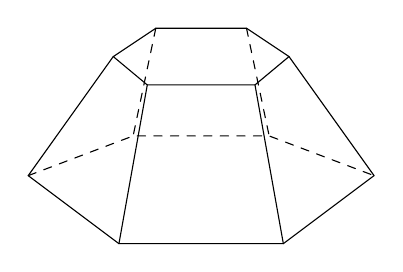
\begin{tikzpicture}[scale=0.72,line cap=round,line join=round]
    \coordinate (T1) at (-1.55,1.55);
    \coordinate (T2) at (-0.80,2.05);
    \coordinate (T3) at (0.80,2.05);
    \coordinate (T4) at (1.55,1.55);
    \coordinate (T5) at (0.95,1.05);
    \coordinate (T6) at (-0.95,1.05);

    \coordinate (B1) at (-3.05,-0.55);
    \coordinate (B2) at (-1.20,0.15);
    \coordinate (B3) at (1.20,0.15);
    \coordinate (B4) at (3.05,-0.55);
    \coordinate (B5) at (1.45,-1.75);
    \coordinate (B6) at (-1.45,-1.75);

    \draw (T1)--(T2)--(T3)--(T4)--(T5)--(T6)--cycle;

    \draw (T1)--(B1);
    \draw[dashed] (T2)--(B2);
    \draw[dashed] (T3)--(B3);
    \draw (T4)--(B4);
    \draw (T5)--(B5);
    \draw (T6)--(B6);

    \draw[dashed] (B1)--(B2)--(B3)--(B4);
    \draw (B4)--(B5)--(B6)--(B1);
\end{tikzpicture}
\end{center}

\end{problem}

\begin{problem}{2004}{2}{3}
A convex quadrilateral $ABCD$ has side lengths $a,b,c,d$, in this order starting from $AB$. Show that if its area is maximal among all such quadrilaterals, then $ABCD$ is cyclic.
\end{problem}

\begin{problem}{2004}{2}{4}
Let $(\mathbf v_1,\mathbf v_2,\dots,\mathbf v_n)$ be an orthonormal basis of $\R^n$. Find the orthogonal complement of
\[
    \Span\{i\mathbf v_i-j\mathbf v_j\mid 1\le i<j\le n\}.
\]
\end{problem}

\begin{problem}{2004}{2}{5}
Let $f\colon[a,c]\to(0,\infty)$ be continuous on $[a,c]$ and differentiable on $(a,c)$. Let
\[
    P=(x_0,f(x_0))
\]
be a point on the graph of $f$. Let $\alpha$ and $\gamma$ be the angles made with the $x$-axis by the lines joining $P$ to $(a,0)$ and $(c,0)$, respectively, and let $\beta$ be the angle made with the $x$-axis by the tangent line to the graph at $P$. Show that there exists $x_0\in(a,c)$ such that
\[
    \tan\alpha+\tan\beta+\tan\gamma=0.
\]
If the tangent line does not meet the $x$-axis, take $\beta=0$.
\end{problem}

\begin{problem}{2004}{2}{6}
Let $f\colon\R\to\R$ be a function whose second derivative $f''$ exists and is bounded on $[0,1]$. Let $(a_n)$ be a sequence such that $0<a_n<1$ for every $n\in\N$, the series
\[
    \sum_{n=1}^{\infty}a_n
\]
diverges, and the series
\[
    \sum_{n=1}^{\infty}a_n^2
\]
converges. If
\[
    \sum_{n=1}^{\infty}f(a_n)
\]
converges, prove that
\[
    \sum_{n=1}^{\infty}|f(a_n)|
\]
also converges.
\end{problem}

\begin{problem}{2004}{2}{7}
Suppose a plane curve $(x(t),y(t))$ of period $T$ satisfies
\[
    \frac{\dd x}{\dd t}=ax-bxy,
    \qquad
    \frac{\dd y}{\dd t}=-cy+dxy,
    \qquad
    x(0)=y(0)=1,
\]
where $a,b,c,d>0$. Find
\[
    \overline{x}\coloneqq\frac1T\int_0^T x(t)\,\dd t,
    \qquad
    \overline{y}\coloneqq\frac1T\int_0^T y(t)\,\dd t.
\]
\end{problem}

\begin{problem}{2004}{2}{8}
Evaluate
\[
    \int_0^{\pi}\frac{x\sin x}{1+\cos^2x}\,\dd x.
\]
\end{problem}

\begin{problem}{2004}{2}{9}
Let $B$ be any $30$-element subset of $\{1,2,\dots,39,40\}$. Prove that there exists a subset $A\subseteq B$ such that
\begin{problemclauses}
    \item $|A|\ge10$;
    \item $x+y\notin A$ for all $x,y\in A$.
\end{problemclauses}
\end{problem}

\begin{problem}{2004}{1}{1}
Let $f\colon\R\to\R$ satisfy
\[
    f(x+y)=f(x)+f(y)
\]
for all $x,y\in\R$. Prove the following.
\begin{problemsubparts}
    \item If $f$ is continuous at $0$, then $f$ is continuous at every $x\in\R$.
    \item If $f$ is continuous on $\R$ and $f(1)=c$, then $f(x)=cx$ for every $x\in\R$.
\end{problemsubparts}
\end{problem}

\begin{problem}{2004}{1}{2}
A frustum of a pyramid has parallel upper and lower bases and uniform density. Find the ratio of the distance from its center of mass to the lower base to the distance from its center of mass to the upper base. The similarity ratio of the upper base to the lower base is $r$, where $r<1$.
\begin{center}
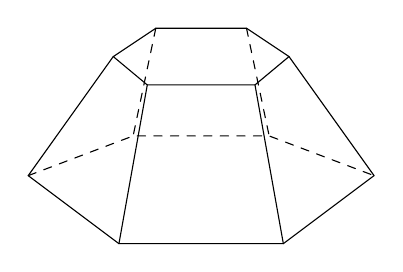
\begin{tikzpicture}[scale=0.72,line cap=round,line join=round]
    \coordinate (T1) at (-1.55,1.55);
    \coordinate (T2) at (-0.80,2.05);
    \coordinate (T3) at (0.80,2.05);
    \coordinate (T4) at (1.55,1.55);
    \coordinate (T5) at (0.95,1.05);
    \coordinate (T6) at (-0.95,1.05);

    \coordinate (B1) at (-3.05,-0.55);
    \coordinate (B2) at (-1.20,0.15);
    \coordinate (B3) at (1.20,0.15);
    \coordinate (B4) at (3.05,-0.55);
    \coordinate (B5) at (1.45,-1.75);
    \coordinate (B6) at (-1.45,-1.75);

    \draw (T1)--(T2)--(T3)--(T4)--(T5)--(T6)--cycle;

    \draw (T1)--(B1);
    \draw[dashed] (T2)--(B2);
    \draw[dashed] (T3)--(B3);
    \draw (T4)--(B4);
    \draw (T5)--(B5);
    \draw (T6)--(B6);

    \draw[dashed] (B1)--(B2)--(B3)--(B4);
    \draw (B4)--(B5)--(B6)--(B1);
\end{tikzpicture}
\end{center}

\end{problem}

\begin{problem}{2004}{1}{3}
A convex quadrilateral $ABCD$ has side lengths $a,b,c,d$, in this order starting from $AB$. Show that if its area is maximal among all such quadrilaterals, then $ABCD$ is cyclic.
\end{problem}

\begin{problem}{2004}{1}{4}
Let $(\mathbf v_1,\mathbf v_2,\dots,\mathbf v_n)$ be an orthonormal basis of $\R^n$. Find the orthogonal complement of
\[
    \Span\{i\mathbf v_i-j\mathbf v_j\mid 1\le i<j\le n\}.
\]
\end{problem}

\begin{problem}{2004}{1}{5}
Let $A$ be the least positive integer of the form
\[
    33^k-7^\ell,
    \qquad k,\ell\in\N,
\]
and let $B$ be the least positive integer of the form
\[
    7^m-33^n,
    \qquad m,n\in\N.
\]
Find $A+B$.
\end{problem}

\begin{problem}{2004}{1}{6}
Let $f\colon\R\to\R$ be a function whose second derivative $f''$ exists and is bounded on $[0,1]$. Let $(a_n)$ be a sequence such that $0<a_n<1$ for every $n\in\N$, the series
\[
    \sum_{n=1}^{\infty}a_n
\]
diverges, and the series
\[
    \sum_{n=1}^{\infty}a_n^2
\]
converges. If
\[
    \sum_{n=1}^{\infty}f(a_n)
\]
converges, prove that
\[
    \sum_{n=1}^{\infty}|f(a_n)|
\]
also converges.
\end{problem}

\begin{problem}{2004}{1}{7}
Suppose a plane curve $(x(t),y(t))$ of period $T$ satisfies
\[
    \frac{\dd x}{\dd t}=ax-bxy,
    \qquad
    \frac{\dd y}{\dd t}=-cy+dxy,
    \qquad
    x(0)=y(0)=1,
\]
where $a,b,c,d>0$. Find
\[
    \overline{x}\coloneqq\frac1T\int_0^T x(t)\,\dd t,
    \qquad
    \overline{y}\coloneqq\frac1T\int_0^T y(t)\,\dd t.
\]
\end{problem}

\begin{problem}{2004}{1}{8}
Let $\mathbf v\in\R^n$ be a unit vector, and let $\mathbf P_{\mathbf v}$ denote the orthogonal projection onto the line $\Span(\mathbf v)$, so that
\[
    \mathbf P_{\mathbf v}\mathbf x=(\mathbf x\cdot\mathbf v)\mathbf v
\]
for every $\mathbf x\in\R^n$. Let $\mathbf A$ be an $n\times n$ positive definite symmetric matrix. Find the maximum value of $\lambda$ such that
\[
    \mathbf A-\lambda\mathbf P_{\mathbf v}\succeq0.
\]
Here $\mathbf B\succ0$ means that every eigenvalue of the symmetric matrix $\mathbf B$ is positive, and $\mathbf B\succeq0$ means that every eigenvalue is nonnegative.
\end{problem}

\begin{problem}{2004}{1}{9}
Let $B$ be any $30$-element subset of $\{1,2,\dots,39,40\}$. Prove that there exists a subset $A\subseteq B$ such that
\begin{problemclauses}
    \item $|A|\ge10$;
    \item $x+y\notin A$ for all $x,y\in A$.
\end{problemclauses}
\end{problem}
